% -*- coding: utf-8 -*-

\chapter{Arquitectura del sistema}

La arquitectura del sistema describe la estructura global del mismo. Incluye su división en componentes, el reparto de responsabilidades entre dichos componentes, la colaboración entre ellos y el flujo de control.
\section{Plataformas de desarrollo y ejecución}

En la realización de este proyecto se ha utilizado una estación de trabajo PC con una configuración de software acorde con las prácticas habituales del grupo de robótica móvil:

\begin{itemize}
  \item Sistema Operativo Windows XP$^{®}$
  \item Lenguaje de programación C++ sobre el entorno de desarrollo MS Visual C++ 6.0$^{®}$ y posteriormente sobre Visual Studio .NET 2005$^{®}$ (Visual Studio 8).
\end{itemize}

Con ello se consigue la compatibilidad con otros trabajos del grupo y se tiene una buena portabilidad del desarrollo. También se ha comprobado que el paso al sistema operativo Windows Vista$^{®}$ es directo y no plantea ningún tipo de problema.

Algunas de las ventajas del lenguaje C++ son su buena capacidad de cálculo, el hecho de que es un lenguaje orientado a objetos y que se trata de un lenguaje de alto nivel con flexibilidad y potencia expresiva. Todo ello permite reducir el tamaño y la complejidad del código. Además, al tratarse de un lenguaje compilado, presenta una buena eficiencia en tiempos de ejecución frente a los lenguajes interpretados. También cabe destacar que gran parte de los entornos de programación distribuidos por los fabricantes de robots móviles están escritos en este lenguaje. Por supuesto, también es compatible con plataformas de desarrollo libre (como la herramienta Player/Stage/Gazebo, que proporciona software gratuito para el desarrollo de aplicaciones con robots y sensores sin imponer un lenguaje de programación determinado).

Respecto al sistema operativo, el uso de Visual Studio impone utilizar Windows. Este entorno simplifica la creación y compilación de código y, sobre todo, permite el tratamiento de cuadros de diálogo e interfaces gráficas para aplicaciones Windows de un modo sencillo. No obstante, son muy abundantes los trabajos en robótica móvil desarrollados con GNU/Linux (Player \& Stage, por ejemplo, no se puede emplear en Windows).

Se han realizado versiones iniciales en modo consola (sobre todo cuando se empleaba simultáneamente el simulador \emph{MobileSim} del robot Pioneer) y finalmente se ha optado por aplicaciones de tipo MFC (\emph{Microsoft Foundation Classes}, ver  \ref{mfc}) basadas en cuadros de diálogo.

El modo de operación puede ser de tipo \emph{simulación}, \emph{fichero} o \emph{real}. La simulación permite observar en pantalla el movimiento teórico de un robot ficticio ante instrucciones que se le dan por medio del ratón o del teclado. Con el modo fichero se muestra de forma similar el comportamiento del sistema al utilizar unos datos de odometría y de medidas del láser guardados previamente en un fichero. El modo real es el que se emplea con el robot verdadero y también permite visualizar los resultados sobre la interfaz gráfica.

Respecto a la plataforma de ejecución para el modo real, en diferentes fases del ciclo de vida del proyecto se han utilizado los robots Pioneer y Urbano. A este último corresponde la implementado el sistema completo y con él se ha llevado a cabo la mayor parte de las pruebas.

En el caso del Pioneer P3AT la puesta en funcionamiento se ha basado en comunicación con cable serie entre un computador portátil y el robot.

Como se ha visto en la introducción, el computador base de Urbano es un PC Pentium con sistema operativo GNU/Linux. También cuenta con un computador secundario que es un PC Pentium con Windows XP. La conexión entre la plataforma de desarrollo y el robot se realiza con un ordenador portátil mediante conexión con el protocolo \emph{telnet} a través de cable Ethernet.

Para más información acerca de estos robots y del resto de hardware utilizado puede consultarse el Anexo \ref{ap:hardware}.

\section{Bibliotecas empleadas}
Para el desarrollo del software del proyecto se ha hecho uso de varias bibliotecas existentes.

\subsection{Standard Template Library (STL)}

Biblioteca de C++ que incluye clases contenedoras, algoritmos e iteradores. Las clases contenedoras son patrones (\emph{templates}) que permiten almacenar objetos de tipos muy variados. Los iteradores son una generalización de los punteros y sirven para acceder a los elementos almacenados en los contenedores. Así, se dice que la STL es una biblioteca \emph{genérica}, ya que sus componentes están altamente parametrizados.

La STL incluye un gran número de algoritmos para manipular los datos guardados en los contenedores. Las funciones que implementan estos algoritmos deberán tomar como argumentos tipos de datos coherentes con las operaciones a realizar. El conjunto de requisitos que debe tener un tipo de dato recibe el nombre de \emph{concepto}. En la STL se definen los siguientes conceptos para clasificar los iteradores: \prog{OutputIterator}, \prog{InputIterator}, \prog{ForwardIterator}, \prog{Bidireccional-} \prog{Iterator}, \prog{RandomAccessIterator}. Algunos de ellos son \emph{refinamientos} de otros, lo que implica una relación similar a la herencia en la programación orientada a objetos.

La clase \prog{vector} es una clase contenedora de tipo secuencial y, como cualquier \emph{template}, puede ser particularizada para contener diferentes tipos de objetos. Se trata de una extensión de los vectores o \emph{arrays} disponibles en C++, con la ventaja de que el número de elementos almacenados puede variar dinámicamente, realizándose la gestión de memoria de forma automática.
Esta clase ha sido ampliamente utilizada en el proyecto.

\subsection{Microsoft Foundation Class Library (MFC)} \label{mfc}

La biblioteca de clases base de Microsoft encapsula gran parte de la API de Windows en clases de C++. Constituye una importante herramienta para desarrollar aplicaciones Windows con entornos de ventanas, menús, etc. Proporciona, entre otras cosas, un gran número de clases para manejar distintos tipos de ventanas predefinidas y para incluir los controles más comunes en cuadros de diálogo.

En el tipo de proyecto empleado se crea una interfaz gráfica constituida por un cuadro de diálogo principal que hereda de la clase pública \prog{CDialog}. Un editor de recursos disponible en Visual Studio facilita la forma de añadir botones al mismo y la declaración de funciones asociadas a los diferentes eventos que pueden tener lugar sobre ellos.

\subsection{Open Graphics Library (OpenGL)}

Biblioteca de funciones estándar para el dibujo de gráficos 2D y 3D. Permite variar los colores, el tamaño y la posición de los objetos, el grosor de las líneas, los focos de luz, los puntos de vista, etc.

En este proyecto se ha utilizado la clase \prog{COpenGLWnd}, implementada por Diego Rodríguez-Losada, como clase base de una nueva clase llamada \prog{CRobot} \prog{MoveGLWnd}. \prog{COpenGLWnd} hereda de la clase \prog{CWnd} de las MFC y permite crear una ventana con fondo negro sobre el que se dibuja una cuadrícula de color magenta y los ejes de un sistema de referencia global para el movimiento sobre un plano. También incluye diversas funcionalidades para cambiar el punto de vista por medio del ratón o el teclado y sirve para dibujar diferentes tipos de robots. En la clase \prog{CRobot\-MoveGLWnd} se maneja el dibujo de trayectorias, obstáculos, puntos del mapa, polígonos\ldots Se ha reprogramado la función virtual \prog{OnKeyDown} de la clase \prog{COpenGLWnd} para modificar las opciones de visualización desde el teclado y para hacer funcionar al robot en modo teleoperado. Desde ella se realiza también el desplazamiento del dibujo del robot de acuerdo con el movimiento del mismo.

\subsection{Biblioteca Mathematics}
Biblioteca desarrollada por Diego Rodríguez-Losada para facilitar el tratamiento de la geometría y distintos tipos de operaciones. En el proyecto se utiliza principalmente para la definición de puntos y segmentos (clases \prog{Point2D} y \prog{Segment2D}). También se dispone de los ficheros \prog{maths.h}, \prog{maths.cpp}, \prog{matrix.h},  \prog{matrix.cpp}, del mismo autor, para definir matrices y operar con ellas.

%Algunas de sus funciones, no obstante, habían sido previamente implementadas en el fichero \prog{tools.cpp}.

\subsection{Biblioteca Aria}

Aria (Advanced Robot Interface for Applications) es una interfaz para el uso de los robots de la firma MobileRobots.Inc que puede usarse sobre las APIs de Linux y Win32. Integra software para establecer las comunicaciones, para controlar la velocidad y la orientación de los robots, para la utilización de diferentes sensores y accesorios\ldots Se trata de una biblioteca escrita en C++, pero también puede ser ampliamente utilizada en Java o Phyton mediante \emph{wrappers}. Se encuentra publicada bajo licencia GPL.

En el proyecto se han utilizado únicamente las funciones básicas que permiten la conexión y desconexión sencilla del robot, el envío de comandos de movimiento de bajo nivel (velocidades de avance y giro) y la lectura de los datos proporcionados por los encóders. La mayor parte de estas funciones se encapsulan dentro de la clases \prog{ArRobot} y \prog{ArSimpleConnector}.

El equivalente a las funciones indicadas ha sido implementado en la clase \prog{CPioneer} para no tener dependencias de Aria fuera de dicha clase.
Además, se utilizan como variables miembro punteros a void, que primeramente se inicializan a NULL para después hacer un cast a vectores que apuntan a los objetos correspondientes (\prog{ArRobot}, \prog{ArSimpleConnector}). Con esto se evita que al ejecutarse la aplicación sea necesario tener instalado el software de Aria.

\section{Funciones auxiliares utilizadas}
A lo largo del desarrollo del proyecto se han creado algunas funciones de carácter auxiliar para realizar ciertas operaciones. Su declaración y contenido se pueden encontrar en los ficheros \prog{tools.h} y \prog{tools.cpp} Las más destacadas son:

\begin{itemize}
  \item \prog{AngRango}: se emplea para convertir un ángulo dado en su equivalente dentro del intervalo
   [-$\pi$, $\pi$].
  \item \prog{ErrAng}: sirve para calcular el ángulo perteneciente a [-$\pi$, $\pi$] que separa un ángulo de partida de un ángulo de destino por el camino más corto.
  \item \prog{Comp}: se utiliza para realizar la composición de dos transformaciones relativas (Ver Anexo \ref{ap:transformaciones}).
  \item \prog{J1}: sirve para calcular la matriz jacobiana de una composición de dos transformaciones relativas respecto de la primera variable  (Ver Anexo \ref{ap:transformaciones}).
  \item \prog{J2}: se emplea para obtener la matriz jacobiana de una composición de dos transformaciones relativas respecto de la segunda variable  (Ver Anexo \ref{ap:transformaciones}).
  \item \prog{eye}: sirve para crear una matiz identidad de las dimensiones que queramos
  \item \prog{InvTrans}: permite calcular la inversión de una transformación relativa entre dos sistemas de referencia  (Ver Anexo \ref{ap:transformaciones}).
\end{itemize}

Las dos primeras funciones resultan de utilidad en el control, la planificación de trayectorias y el control reactivo. El resto se utilizan principalmente para la localización y en el tratamiento de los mapas.

\section{ Estructura de clases}
En la figura \ref{fg:uml} se puede ver el diagrama UML de las clases que conforman el sistema.

\begin{figure}[tbp]
  \centering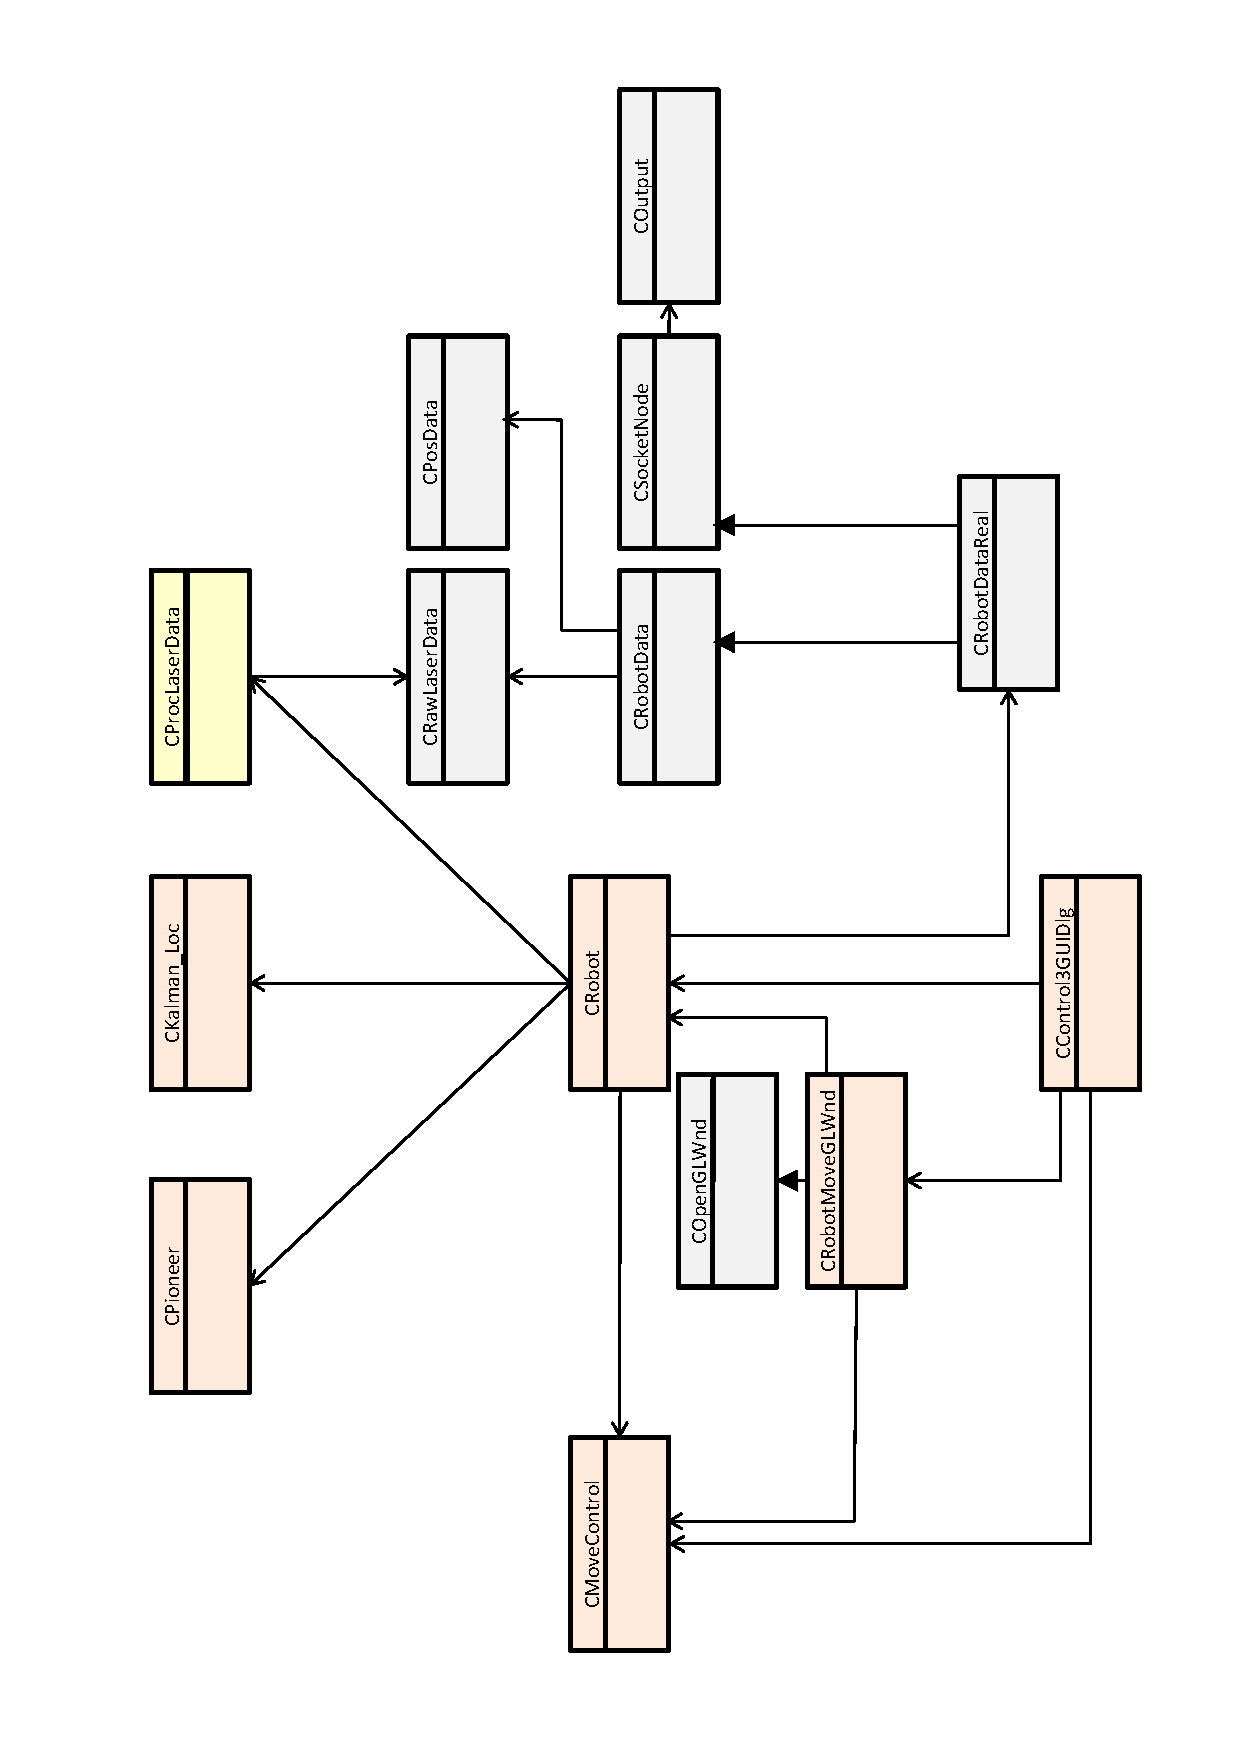
\includegraphics[scale=0.65]{clases4}\\
  \caption{Diagrama de clases del sistema}\label{fg:uml}
\end{figure}

En el diagrama no se muestran las dependencias de las bibliotecas anteriormente descritas. Como puede observarse, se ha realizado un diseño modular con relaciones claras entre sus elementos. Las clases que han sido implementadas en el presente proyecto aparecen en color rosa. El color gris se ha utilizado para las clases que existían previamente. La clase \prog{CProcLaserData} forma parte de este último grupo, pero ha sido ligeramente modificada.

A continuación se explica el uso que se ha hecho de estas clases mientras que las clases nuevas serán tratadas en posteriores capítulos, después de que se estudien los algoritmos incorporados.

\subsection{La clase \prog{CRawLaserData}}
Esta clase se encarga principalmente de leer y escribir ficheros con los datos procedentes del láser y de ajustar dicha información al formato correspondiente para ser enviada o tras ser recibida por un socket. También define una macro con el máximo número de medidas que puede proporcionar el láser, igual a 361.
Sus métodos son los siguientes:

\subsubsection{\prog{Load}}

\noindent
\prog{int Load(FILE* source\_file)}

\noindent
Esta función se emplea para leer de un fichero los datos correspondientes a las medidas del láser.

\begin{itemize}
  \item \prog{source_file}: fichero del que se lee la información del láser
\end{itemize}

\noindent
Los resultados obtenidos sobre el instante en que se efectúa la medida, el identificador del láser, el número de medidas, el ángulo recorrido por éste y su resolución y el máximo alcance del láser se almacenan en variables con nombres representativos: \prog{time_stamp\_seconds}, \prog{time_stamp_useconds}, \prog{id_laser}, \prog{num_med}, \prog{scan_angle}, \prog{scan_resolution}, \prog{max_range}\ldots

Estos datos han de ir seguidos de dos puntos, :, y detrás han de aparecer las medidas sucesivas de las distancias asociadas a cada ángulo, que se van guardando en el vector de enteros \prog{med}. Todos los valores deben ir separados por un espacio en blanco para ser leídos correctamente. En el ejemplo de la figura \ref{fg:ficherolaser} puede verse mejor cómo ha de ser el formato de una línea del fichero:

\begin{figure}[h]
  % Requires \usepackage{graphicx}
  \centering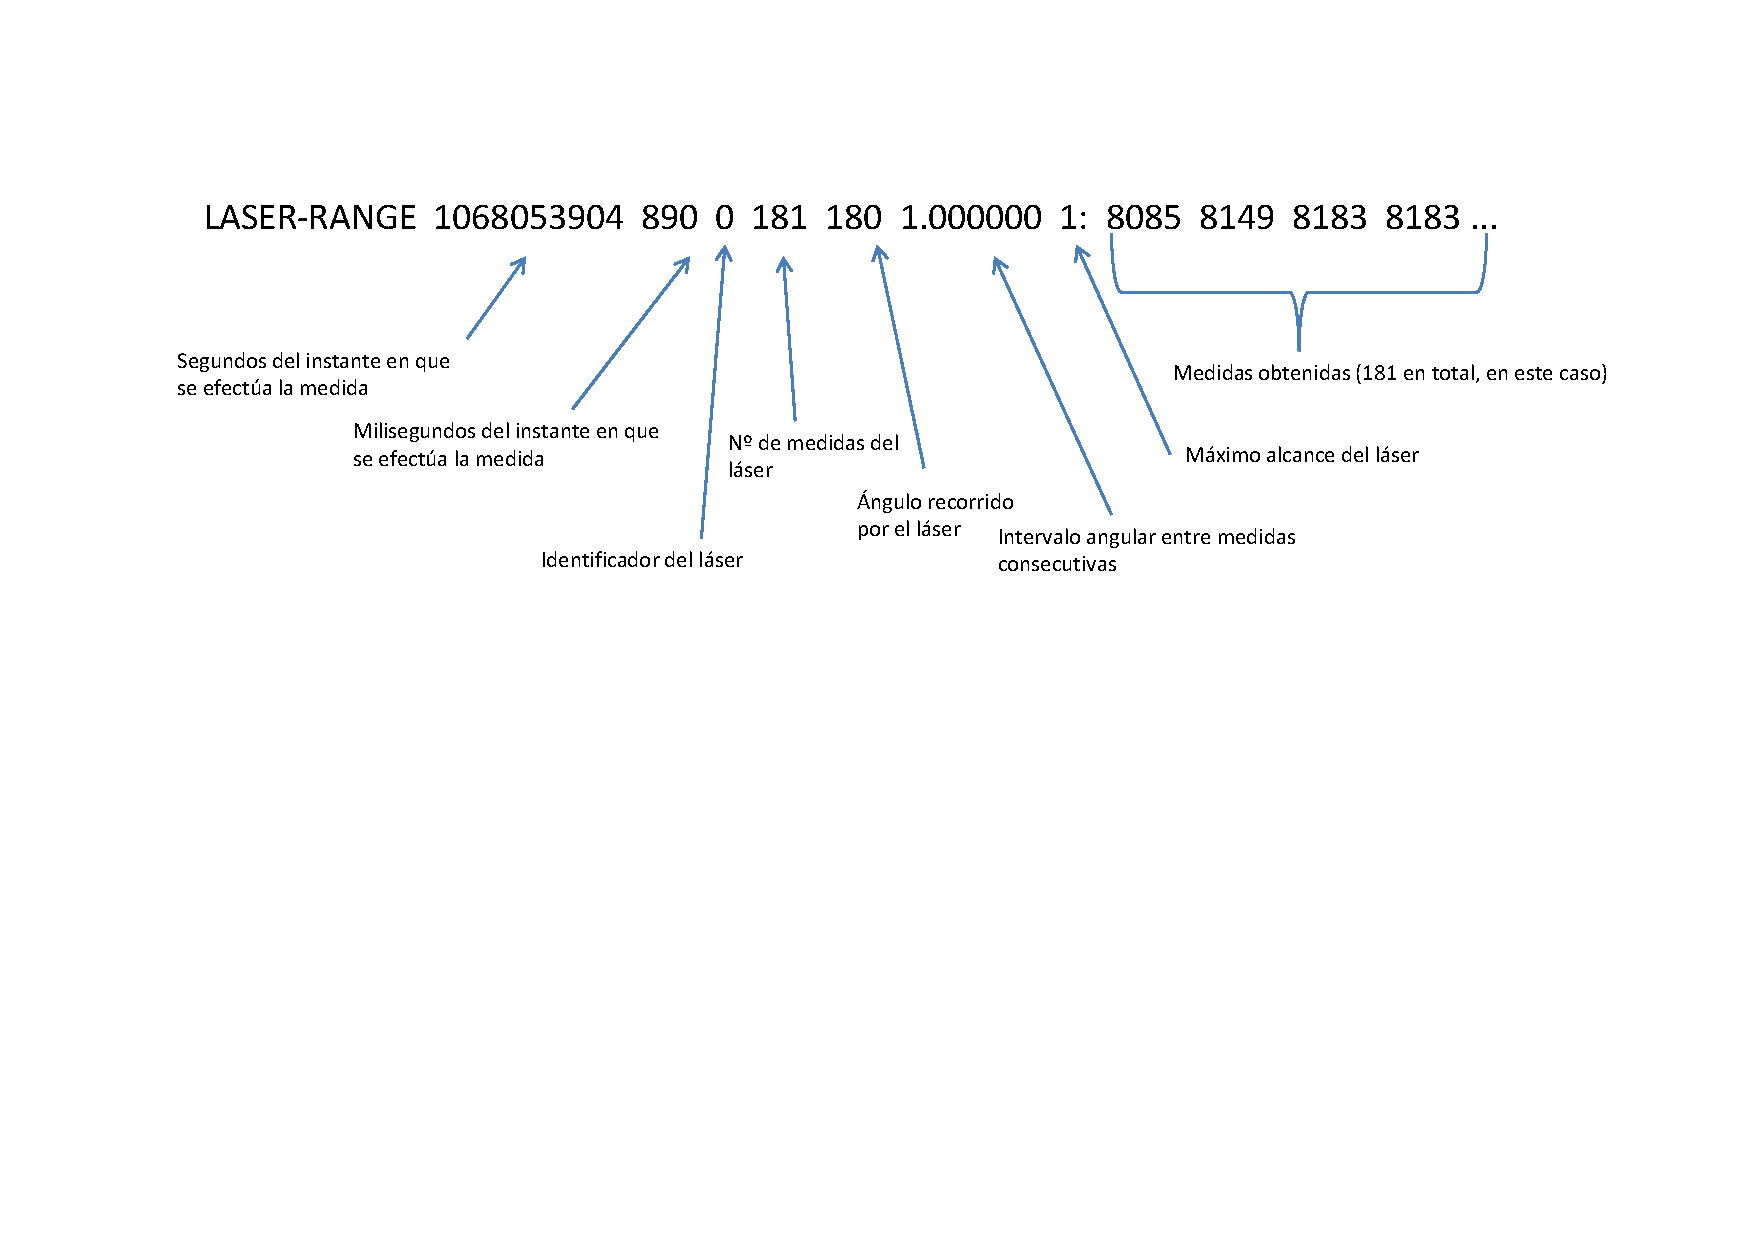
\includegraphics[width=0.9\textwidth]{laserfichero}\\
  \caption{Línea de fichero correspondiente a datos del láser}\label{fg:ficherolaser}
\end{figure}

\noindent
Si hay algún fallo en la lectura de los parámetros o de las medidas se devuelve $-1$. Si el fichero tiene el formato adecuado y se lee sin ningún problema se devuelve $0$.

\subsubsection{\prog{Save}}

\prog{void Save(FILE* log\_file)}

\noindent
Esta función se emplea para escribir en un fichero los datos correspondientes a las medidas del láser.

\begin{itemize}
  \item \prog{log\_file}: fichero en el que se escribe la información del láser
\end{itemize}

\noindent
Se escribe el término LASER\_RANGE seguido del contenido de las variables \prog{time_stamp_seconds}, \prog{time_stamp_useconds}, \prog{id_laser}, \prog{num_med}, \prog{scan_angle}, \prog{scan\_resolution)} y \prog{max\_range} y dos puntos (':'). Después se escriben los valores de las diferentes medidas almacenadas en el vector \prog{med}. Todos los datos van separados por un espacio en blanco. En resumen, una llamada a esta función escribe una línea de fichero con el formato mostrado en \ref{fg:ficherolaser}.

\subsubsection {\prog{Serialize}}
\prog{int Serialize(char* cad,int\& l,int size) const}
\subsubsection {\prog{DeSerialize}}
\prog{int DeSerialize(char* cad,int\& l,int size)}

\vspace{0.2cm}
\noindent
Estas dos funciones no se han utilizado directamente, por lo que no se entra en detalles sobre su funcionamiento.

\subsection{La clase \prog{CProcLaserData}}
Se trata de una clase para el procesamiento y manejo de la información del láser. Sus métodos más utilizados son:

\subsubsection {\prog{SetOffset}}

\prog{void SetOffset(float offx, float offy, float offz)}

\noindent
Esta función se emplea para establecer el offset del láser, es decir, indica la posición del mismo respecto al sistema de referencia local del robot.

\begin{itemize}
  \item \prog{offx}: desplazamiento del láser sobre la coordenada x del sistema de referencia local del robot
  \item \prog{offy}: desplazamiento del láser sobre la coordenada y del sistema de referencia local del robot
  \item \prog{offz}: desplazamiento del láser sobre la coordenada z del sistema de referencia local del robot
\end{itemize}

\noindent
En el robot Urbano el offset del láser viene dado por (0.168, 0.0, 1.2) y en el Pioneer P3AT los valores son (0.0, 0.0, 0.4).

Estos parámetros se pasan a las variables miembro \prog{off\_x}, \prog{off\_y} y \prog{off\_z}. Además, en ella se calculan las razones trigonométricas seno y coseno de los ángulos correspondientes a todas las diferentes medidas que pueden tomarse (intervalos de $0,5º$) y se guardan en sendos vectores \prog{cos\_alfa} y \prog{sen\_alfa}, de tamaño igual al máximo número de medidas posibles.

\subsubsection {\prog{DefineData}}

\prog{int DefineData(const CRawLaserData\& d)}

\noindent
Permite calcular las coordenadas de los puntos correspondientes a las medidas del láser.

\begin{itemize}
  \item \prog{d}: objeto de la clase \prog{CRawLaserData} cuyos datos se van a procesar
\end{itemize}

\noindent
A partir del alcance de las medidas realizadas se ajusta el valor de las distancias hasta los obstáculos sobre cada ángulo de medida (almacenadas en el vector \prog{med}) y el resultado se guarda en un vector de enteros de nombre \prog{fmed}.
\noindent
Con el offset del láser y dichas medidas de distancia se obtienen las coordenadas de cada punto $i$ detectado mediante trigonometría:

\begin{eqnarray*}
\mbox{med\_x}[i] &= &\mbox{off\_x}+\mbox{fmed}[i]\mbox{cos\_alfa}[istep] \\
\mbox{med\_y}[i] &= &\mbox{off\_y}+\mbox{fmed[}i]\mbox{sen\_alfa}[istep] \\
\mbox{med\_z}[i] &= &\mbox{off\_z}
\end{eqnarray*}

\noindent
donde el valor de la variable \prog{step} puede ser $1$ ó $2$, viniendo dado por el número de medidas. De este modo se toman los ángulos de $0,5º$ en $0,5º$ o de $1º$ en $1º$.
\noindent
Los puntos 2D que así se obtienen (la coordenada $z$ se mantiene constante) se almacenan en el vector de la STL \prog{v}, miembro de esta clase.

La función devuelve un $0$ si el número de medidas es distinto de $181$ o de $361$ (en cuyo caso no se realiza procesamiento de las medidas, ya que ha de haber algún error) y un $1$ cuando el número de medidas es el adecuado y, por lo tanto, se han efectuado todas las operaciones de la definición de datos.

%subsection {AsignaParamLineSplit}
%
%prog{void AsignaParamLineSplit(float max_dis,float min_leng,int min_poin,float max_alcan,float max_sep)}
%
%signación de una serie de parámetros empleados para el cálculo de un polígono de puntos mediante el procedimiento que se indica en \ref{poligono}.
%
%begin{itemize}
% \item \prog{max_dis}:
% \item \prog{min_leng}:
% \item \prog{min_poin}:
% \item \prog{max_alcan}:
% \item \prog{max_sep}:
%end{itemize}
%
%Los valores utilizados con el robot Urbano son:
%prog{max_dis} $= 0.025$
%prog{min_leng} $= 0.6$
%prog{min_point} $= 11$
%prog{max_alcan} $= 8.0$
%prog{max_sep} $= 0.2$

\subsection{La clase \prog{CPosData}} \label{CPosData}

Esta clase es similar a la clase prog{CRawLaserData} pero se encarga del tratamiento de la información referente a la odometría. Dispone de variables miembro públicas en las que almacenar la posición odométrica y las velocidades del robot (\prog{posx}, \prog{posy}, \prog{posth}, \prog{vel_drive}, \prog{vel_steer}). Sus métodos son:

\subsubsection{\prog{Load}}

\noindent
\prog{int Load(FILE* source\_file)}

\noindent
Esta función se emplea para leer de un fichero los datos correspondientes a las medidas de odometría.

\begin{itemize}
  \item \prog{source_file}: fichero del que se lee la información de la odometría
\end{itemize}

\noindent
Los resultados obtenidos sobre el instante en que se efectúa la medida, la coordenadas $x, y$ y $z$ de la posición, la velocidad de avance y la velocidad de giro se almacenan en las variables correspondientes: \prog{pos_temp}, \prog{pos_time_ms}, \prog{posx}, \prog{posy}, \prog{posth}, \prog{vel_drive} y \prog{vel_steer}.

En el ejemplo de la figura \ref{fg:ficheropos} se muestra cómo ha de ser el formato de una línea del fichero:

\begin{figure}[h]
  % Requires \usepackage{graphicx}
  \centering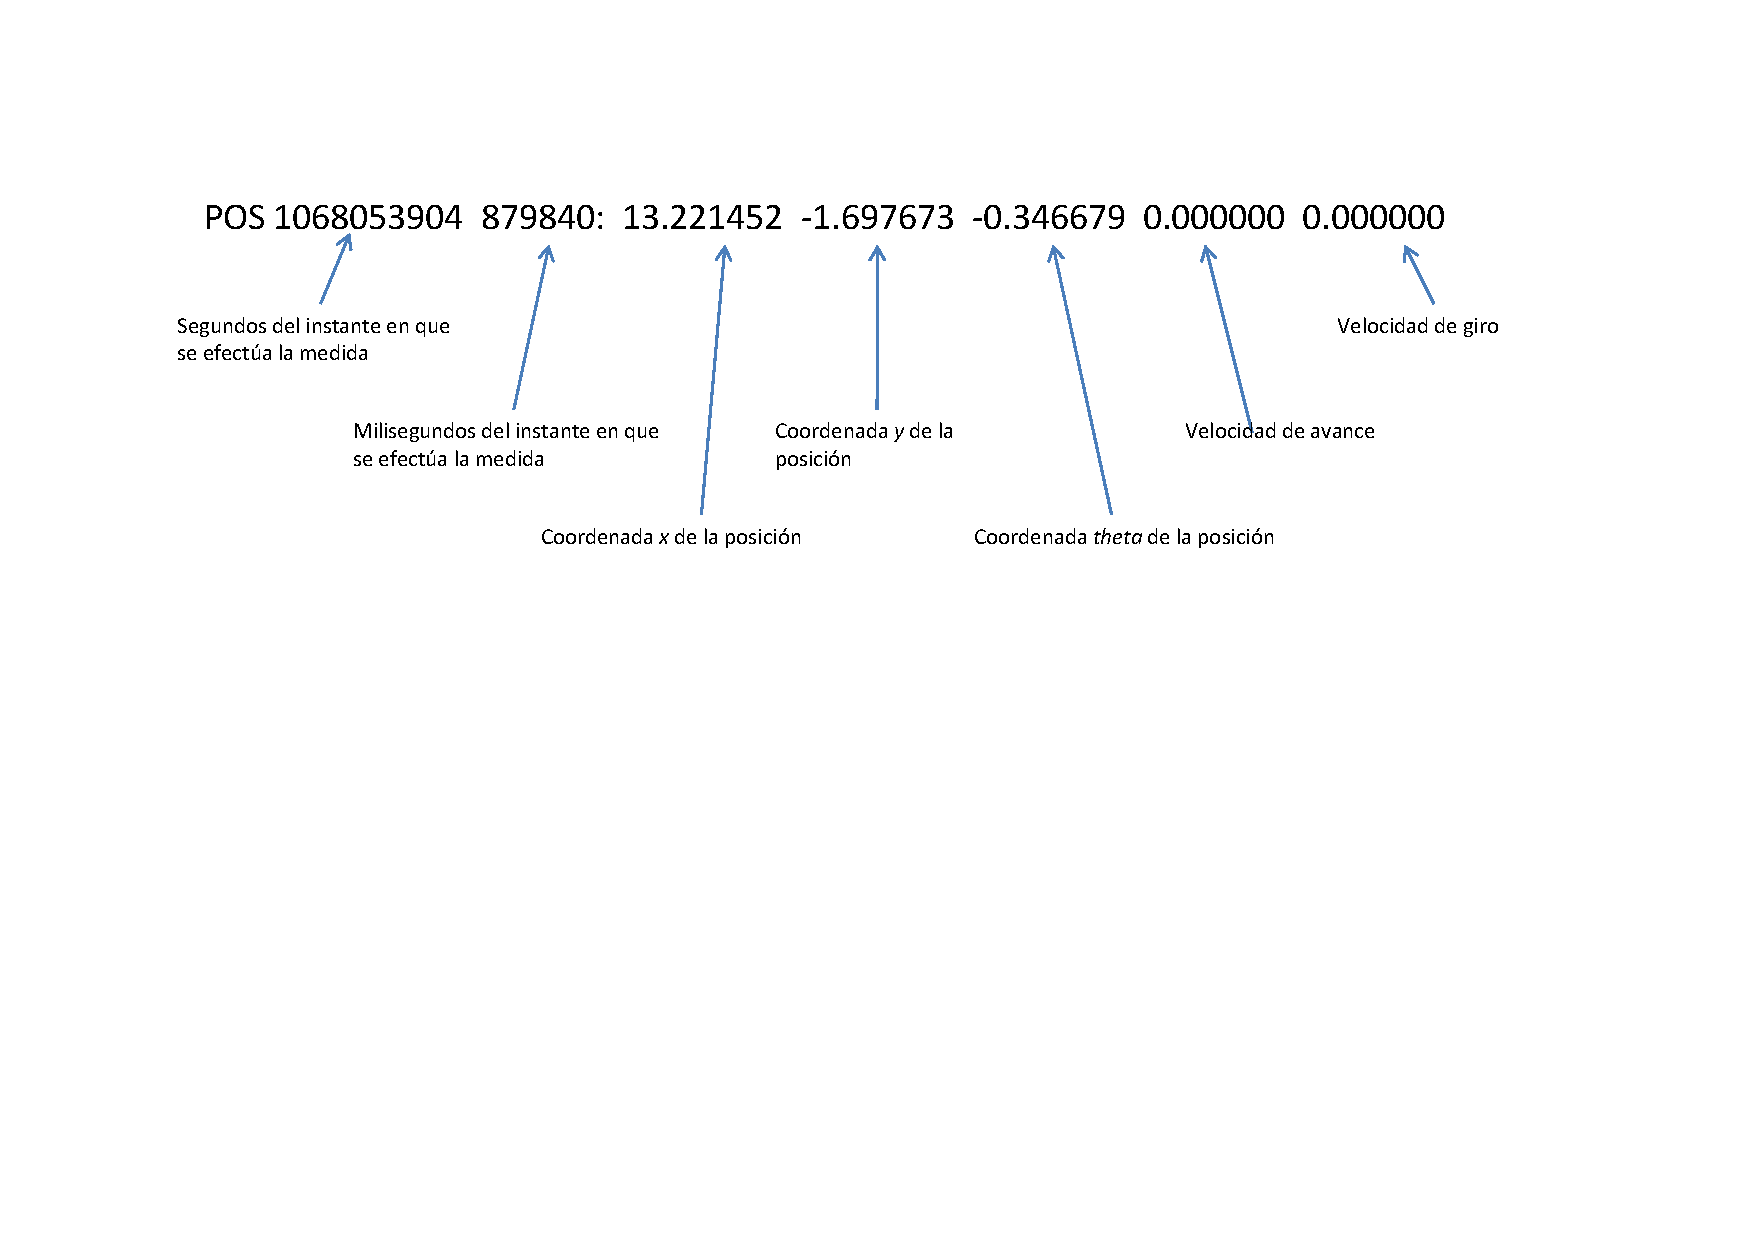
\includegraphics[width=0.9\textwidth]{posfichero}\\
  \caption{Línea de fichero correspondiente a datos de odometría}\label{fg:ficheropos}
\end{figure}

\noindent
Si hay algún fallo en la lectura de los parámetros o de las medidas se devuelve $-1$. Si el fichero tiene el formato adecuado y se lee sin ningún problema se devuelve $0$.

\subsubsection{\prog{Save}}

\prog{void Save(FILE* log\_file)}

\noindent
Esta función se emplea para escribir en un fichero los datos correspondientes a las medidas de posición.

\begin{itemize}
  \item \prog{log\_file}: fichero en el que se escribe la información de la odometría
\end{itemize}

\noindent
Se escribe el término POS seguido del contenido de las variables \prog{pos_temp} y \prog{pos_time_ms} y dos puntos (':'). Después se escriben los valores de \prog{posx}, \prog{posy}, \prog{posth}, \prog{vel_drive} y \prog{vel_steer}. Todos los datos van separados por un espacio en blanco. En resumen, una llamada a esta función escribe una línea de fichero con el formato mostrado en \ref{fg:ficheropos}.

\subsubsection {\prog{Serialize}}
\prog{int Serialize(char* cad,int\& l,int size) const}
\subsubsection {\prog{DeSerialize}}
\prog{int DeSerialize(char* cad,int\& l,int size)}

\vspace{0.2cm}
\noindent
Al igual que en la clase \prog{CRawLaserData}, estas dos funciones no se han utilizado directamente, por lo que no se entra en detalles sobre su funcionamiento.

\subsection{La clase \prog{CRobotData}}
Esta clase se emplea para definir en cuál de los tres modos posibles se ha de conectar el robot y para procesar la información que permite su funcionamiento en los modos \emph{simulación} y \emph{fichero}. En ella se definen una serie de macros para indicar tipos de conexión (\prog{SIMU_CONN}, \prog{FILE_CONN}, \prog{REAL_CONN}) , tipos de datos (\prog{DATA_CONN_ERROR}, \prog{DATA_NONE}, \prog{DATA_ODOM}, \prog{DATA_LASER}, \prog{DATA_ODOM_LASER}, \prog{DATA_ODOM_INIT}) y tipos de estado (\prog{STATUS_NOT_INIT}, \prog{STATUS_CONNECTION_} \prog{ERROR}, \prog{STATUS_CONNECTED}. Dentro de la clase se tienen dos variables miembro para el manejo de los datos de la odometría y del láser: \prog{odom_data}, de la clase \prog{CPosData}, y \prog{laser_data}, de la clase \prog{CRawLaserData}. Las principales funciones que se utilizan son las siguientes:

\subsubsection{\prog{Init}}

\noindent
\prog{bool Init(int typ,const char* source)}

\noindent
Esta función se define como \prog{virtual} (para que pueda reescribirse en clases que hereden de ésta) y se emplea para establecer el modo de funcionamiento del robot. En caso de que el modo sea tipo fichero también se abre el fichero del que han de leerse los datos.

\begin{itemize}
  \item \prog{typ}: modo de funcionamiento del robot
  \item \prog{source}: nombre del fichero de datos o IP del robot real al que ha de conectarse el sistema
\end{itemize}

\noindent
En primer lugar se copia el parámetro \prog{source} en la cadena \prog{source_name}, variable miembro de la clase. Si la conexión es de tipo fichero, se abre el fichero de nombre \prog{source_name} en modo lectura. Si el fichero no existe la función devuelve \prog{false}. En caso contrario se guarda el modo de funcionamiento en la variable entera \prog{type}, también miembro de la clase, con los posibles valores \prog{FILE_CONN} (1), \prog{SIMU_CONN} (2) o \prog{SIMU_REAL} (3) y la función devuelve \prog{true}.

\subsubsection{\prog{SpeedValues}}

\noindent
\prog{void SpeedValues(float vel_drive, float vel_steer)}

\noindent
Esta función se emplea para ajustar las velocidades al formato y rango adecuados.

\begin{itemize}
  \item \prog{vel_drive}: velocidad de avance que se le quiere dar al robot
  \item \prog{vel_steer}: velocidad de giro que se le quiere dar al robot
\end{itemize}

\noindent
Si la velocidad de avance es superior a 100 se le da valor 100 y si es menor que 0 se le da valor 0. Con la velocidad de giro se hace lo mismo en el intervalo [-100,100]. Ambos resultados se convierten a tipo \prog{char} y se almacenan en las variables de clase \prog{com_drive} y \prog{com_steer}.


\subsubsection{\prog{LoadData()}}

\noindent
\prog{int LoadData()}

\noindent
Esta función se emplea para leer de un fichero los datos correspondientes a las medidas de odometría o del láser.

\noindent
En líneas generales, se lee la primera palabra de la línea del fichero abierto en la llamada a \prog{Init} en la que estemos y se mira si es igual a las cadenas "POS" o "LASER-RANGE". En el primer caso, se llama a la función \prog{Load} sobre el objeto \prog{pos_data} y en el segundo, a la función \prog{Load} del objeto \prog{laser_data}.

\noindent
Se devuelve el tipo de datos obtenido (\prog{DATA_CONN_ERROR}, \prog{DATA_ODOM}, \prog{DATA_} \prog{LASER}\ldots).

\subsubsection{\prog{Simulate}}

\noindent
\prog{int Simulate()}

\noindent
Esta función se emplea para actualizar la información de la odometría y del láser en el modo simulación.

\noindent
Respecto a la odometría, su actualización se realiza mediante composición de la posición odométrica anterior (accesible mediante \prog{odom_data}) con un vector de incrementos definido a partir de las velocidades \prog{com_drive} y \prog{com_steer}. Esta nueva posición obtenida se emplea para actualizar las variables \prog{posx}, \prog{posy} y \prog{posth} de \prog{odom_data}, de forma que queda disponible para la siguiente llamada. En lo relativo al láser, en la simulación se establece que el número de medidas es 181, que el ángulo que se cubre es de 180º, que las medidas se toman cada 1º y que el valor de todas ellas es \prog{laser_data.med[i]} $= 8000$ (límite de alcance).

\noindent
El valor que se devuelve es siempre \prog{DATA_ODOM_LASER}.

\subsubsection{\prog{UpdateData}}

\noindent
\prog{int UpdateData()}

\noindent
Esta función es de tipo \prog{virtual} y se emplea para actualizar los datos de la odometría y del láser en los modos simulación y fichero.

\noindent
Si el tipo de conexión es \prog{FILE_CONN} se efectúa una llamada a la función \prog{LoadData}. Si el tipo de conexión es \prog{SIMU_CONN} se llama a la función \prog{Simulate}. En estos casos se devuelve el resultado de estas llamadas. Por defecto se devolverá \prog{DATA_CONN_ERROR} (tras realizarse la actualización del estado a \prog{STATUS_} \prog{CONNECTION_ERROR}).

\vspace{0.2cm}
Otras funciones de la clase que se utilizan para guardar en un fichero los datos de la odometría y del láser son \prog{StartLogData} (crea y abre el fichero en el que escribir los datos), \prog{Log} (que a su vez llama a las funciones \prog{Save} de las variables \prog{odom_data} o \prog{laser_data} según corresponda) y \prog{StopLogData}.

\subsection{La clase \prog{CSocketNode}}
Es la clase encargada de establecer las comunicaciones con el robot real mediante el uso de sockets. No se ha utilizado directamente.

\subsection{La clase \prog{CRobotDataReal}}
Como se puede ver en el diagrama \ref{fg:uml}, esta clase hereda de \prog{CRobotData}y \prog{CSocketNode}. Es la clase necesaria para el funcionamiento del robot en modo real. Sus métodos más importantes son los siguientes:

\subsubsection{\prog{Init}}

\noindent
\prog{bool Init(int typ,const char* source)}

\noindent
Esta función se emplea para establecer el modo de funcionamiento del robot y efectuar la conexión en el caso de modo real.
\begin{itemize}
  \item \prog{typ}: modo de funcionamiento del robot
  \item \prog{source}: nombre del fichero de datos o IP del robot real al que ha de conectarse el sistema
\end{itemize}

\noindent
En ella se hace una llamada a la función \prog{Init} de la clase \prog{CRobotData}, de forma que sólo es necesario añadir la funcionalidad de establecer conexión en modo real. En ese caso, se leen del parámetro \prog{source} la dirección IP y el puerto de escucha del servidor con el que se ha de realizar la conexión. Una vez se tienen estos datos, se inicia un socket cliente y se lanza el thread que se encarga de la comunicación entre éste y el servidor. Para ello se utilizan funciones de \prog{CSocketNode}. El valor de retorno es siempre \prog{true}.

\subsubsection{\prog{TransferData}}

\noindent
\prog{int TransferData()}

\noindent
Esta función se emplea para enviar los valores de velocidad al robot y recibir de él la información sobre la odometría y las medidas del láser.

\noindent
Los datos de velocidad se envían en el formato "TransferData 100 -10", donde 100 sería la velocidad de avance y -10, la velocidad de giro. Los datos de odometría y del láser que se reciben se pasan a las variables \prog{odom_data} y \prog{laser_data} por medio de sus métodos \prog{DeSerialize}, de modo que quedan procesados para su utilización en el resto del programa.


\subsubsection{\prog{UpdateData}}

\noindent
\prog{int UpdateData()}

\noindent
Esta función se emplea para actualizar los datos de la odometría y del láser en el modo real.

\noindent
Si el tipo de conexión es \prog{REAL_CONN} se efectúa una llamada a la función \prog{TransferData} y posteriormente a \prog{Log} para guardar los datos obtenidos en un fichero (siempre que previamente se haya empleado \prog{StartLogData}). En caso contrario (\prog{SIMU_CONN} o \prog{FILE_CONN}) se llama a la función \prog{Update} de la clase \prog{CRobotData}.

\noindent
Se devuelve el tipo de datos obtenido (\prog{DATA_CONN_ERROR}, \prog{DATA_ODOM}, \prog{DATA_} \prog{LASER}, \prog{DATA_ODOM_LASER} o \prog{DATA_NONE}).



